%\pagestyle{article}
\documentclass[a4paper]{article}
\usepackage[english]{babel}
\usepackage[utf8]{inputenc}
\usepackage{graphicx} % for figures
\usepackage[section]{placeins} %This prevents placing floats before a section.
\usepackage{csquotes}

\usepackage{natbib}% better citation
\usepackage{hyperref} %autoref

%% Sets linestretch, paragraphstrech, indentation and footnote stuff 
\usepackage{parskip} %space between paragraphs
\parskip=12pt %set space between paragraphs
\setlength\parindent{12pt} %paragraf indentation
\usepackage[onehalfspacing]{setspace} %linespacing; does not affect footnotes
\setlength{\footnotesep}{0.7\baselineskip}% space between footnotes
\usepackage[hang,flushmargin]{footmisc} %% removes identation in footnoteshttps://www.overleaf.com/project/5b98e00a21d3bd15ac5a2e86

\usepackage{makecell} % make cells in tabels for longer text

\usepackage[colorinlistoftodos]{todonotes}

%% For header and footer (1)
% Marco
\usepackage{fancyhdr}
\pagestyle{fancy}
\textwidth = 424pt % test width ish
\oddsidemargin = 18pt % margin width ish

\fancyheadoffset{0 in} % Shifty solutions..

\fancyhf{} %% clear defuelt header and footer

%% For header and footer (2)
%Specifics
\lhead{Simon P. von der Maase}
\rhead{\today}

\lfoot{University of Copenhagen}
\rfoot{\thepage}
\renewcommand{\footrulewidth}{0.8pt}

\title{A Morden Approach to Conflict Prediction\\or: Dude, Here's Your Conflict\\ or: Where Men Rebel}

\author{Simon Polichinel von der Maase}
\date{September 2018}

\begin{document}

	\begin{titlepage}
		\maketitle
		\noindent\rule{\linewidth}{0.4pt}
		\begin{figure}[h]
			\centering
			
\includegraphics[scale=0.32]{KU_logo.png}
		\end{figure}
		\thispagestyle{empty} % removes page number on front page
	\end{titlepage}
    \tableofcontents
\pagebreak

\begin{abstract}
\todo[inline]{To come..}
\end{abstract}
\pagebreak

\section{Introduction}
%\subsection{The 'What'}

% Du har ikke data med fra efter 2010 fordi den igen der bliver for ufuldstændig..

Humans kill humans - a lot of humans. In 2009 alone an estimated 46,772 people where killed over the course of 6194 incidents of internal conflicts\footnote{according to the best estimate from the Uppsala Conflict Data Program}. The number of lives ruined as a consequence of these killings no doubt exceeds the number of deaths by magnitudes. Even far away from the conflict zones countries experience the consequences of conflict - not least in the form large influx of refuges and the insuring political turmoil. The long term solution to the this senseless onslaught probably involves some fundamental changes to the global power structures involving the cooporation of the global political, economic and cultural elites alike. However, while we wait for this to happen, another, less Utopian approach is to mitigate this ongoing catastrophe by creating a reliable "early warning system". A predictive framework capable of estimating the probability that a given geographic location will experience conflict during a given time period. Using this information governments, ngo's or other responsive actors can act to prevent the conflict, mitigate the fallout, or secure civilians. Naturally, such intervention are both disruptive and expensive. Thus for any predictive framework to work as a practical early-warning-system a high level of accuracy is needed; we need to ensure that the geographic locations which are being appointed the highest risk by the framework is indeed where future conflicts are most likely to occur.\par

This paper presents a modern computational approach to conflict prediction and forecasting. It is constructed as a unified framework to asses the probability that a given sub-national geographical location will experience battle-related deaths as a consequence of intra-state conflict. The challenge is handled as a forecasting problem, thus the prediction target is whether or not the given location experiences any battle-related deaths \emph{next year}. The given geographical unit is a PRIO-grid cell, which is a cell of $0.5\times0.5$ decimal degrees. I am not trying to estimate the number of deaths; only the presence of deaths. Thus the target is binary, taking either the value of 1 or 0 with 1 denoting the presence of fatal conflict. Importantly, however, the estimate will not be binary but probabilistic.\par

This is a preliminary project, thus the aim is as much to explore fruitful approaches and methods for future research as it is making good predictions. As a consequence a lot of this paper is dedicated to choosing what goes into the model and not least evaluating what comes out.\par

The model itself consists of an large ensemble of Extreme Gradient Boosting classifiers (xgboost), which is an special boosting algorithm based on ensembles of regression tress well suited for both large date-sets and rare events detection.\par

What goes in to the model is a roster of features derived from both the theoretical and empirical literature regarding civil wars and intra-state conflicts. The relationship does not need to be causal, but I do demand a salient theoretical link between the target and the features, thus insuring usefulness of the feature in a practical long-term forecasting scenario.\par

What comes out of the model is first of all probabilities of conflict deaths pertaining to a given geographical cell in a given year, wich are evaluated against the actual observations. But just as importantly the framework allows for evaluation of the individual features importance in the prediction process. This insight is paramount when deciding how to improve the framework and where to invest resources in future endeavours.\par

% ----------------------------------------------------------------------

\todo[inline]{Det her under skal skrives om til at matche evalueringen}
The model constructed is remarkable reliable in out-of-sample prediction with an AUC (ROC) of XX. Even more impressive is the fact that i captures all most all events, with a recall of XXXX when applying a threshold of 0.5 - that is when I classify all events with a predicted probability of conflict above 0.5 as conflicts. Unfortunately, when faced with the unbalanced nature of the real world the model do generate relatively many false positives as underscored with a precision at XXXX and an average precision (precision recall curve) of XXXX. Never-the-less the model does reach a accuracy of XXXX; and that is while still capturing most of the rare events. Presented in a less technical jargon: If I categories all predictions with a probability of conflict of 0.5 or above as predicted conflicts then given all the conflicts - pertaining to some given year - my model will on average correctly classify XXXXX\%(recall) of the conflicts which will occur the following year. However these events only make op XXXX\% of events classified by the models as conflicts. Thus, I do predict a more dangerous world then we actual do live in. Still while the number of false positives is rather high compared to true positives it is rather low compared to the total number of observations and thus model is over all correct in its assessment XXXXX\% (accuracy) of the time.\par

\todo[inline]{Skal også lige tjekkes til sidst.}
The Features credited with most of the prediction power are generally features pertaining directly to the temporal and spatial dimensions of conflict; how far is a cell from the nearest conflict; How many conflicts have the cell previous seen; How many fatalities where 'this' year reported in the country which the cell belongs to ect.. This is followed by features pertaining to the population size of the cell and the size of the country which the cell belongs to. Then grievance based features enters; such as whether the cell is economically deprived relative to the country as a whole and whether the cell is inhabited by politically excluded ethnic groups. Lastly come features pertaining to greed and resources such as absolute economic capacity and the presence of oil.\par

% ----------------------------------------------------------------------

Going forward with future endeavours I recommend allocating resources to create a more unified and systematic framework modeling the temporal-spatial evolution of conflicts as a function of it self. For one thing it seems the most productive way to improve prediction power, but just as important the conflict data are more often updated and the last entry closer to the present year then the contextual features used in this project. Thus the conflict data itself presents itself as better suited for real life forecasting applications. Such a framework would also constitute an appropriate baseline-model which could be used to evaluate the relevance of new features and feature specifications.\par

The to following sections will first present the motivation and then the research question and design. This is followed by a introduction to the data sources and a presentation of the included features. Next I present the predictive framework and a thorough analysis of the derived results. This is proceeded by a discussion regarding future challenges and suggestions for improvements. Lastly a conclusion sums up the main findings.\par

\subsection{The 'Why'}

\begin{displayquote}
\emph{[...] the estate of Man can never be without some incommodity or other; and [...] the greatest, that in any form of Government can possibly happen to the people in generall, is scarce sensible, in respect of the miseries, and horrible calamities, that accompany a Civill Warre;} \cite[128]{Hobbes_1991}  \par

\end{displayquote}

The perils and miseries of civil war and internal conflict have plague mankind all throughout history. Presumably intra-state conflicts have been around as long as there have been states to exercise conflict within - and the last century has been no exception. Since the conclusion of the Second World War intra-state conflicts have been far more common then inter-state wars \citep[563]{Collier_Hoeffler_2004}; Over five times as many people have died in intra-state conflicts compared to inter-state wars \citep[563]{Collier_Hoeffler_2004}; and since 1960 over one half of all nations have experienced some sort of violent internal conflict leading to fatalities \citep[3-4]{Blattman_Miguel_2010}.\par

Importantly, internal conflicts should not be viewed as internal affairs of little concern to other then the inflicted host and its allied. Examples of spillover effects facilitating the spread of conflicts across boarders a ample. At country level, having a country located in a conflict ridden neighbourhood have been shown to be a robust predictor of internal conflict \citep{Hegre_Sambanis_2006,Goldstone_2010}. Internal conflict is thus a highly destructive and potentially contentious malaise only to be ignored by the most imprudent or hostile observers. Understanding how internal conflicts originates and spreads in order to prevent or mitigate the destruction is indeed as crucial as ever.\par

Encouragingly, developments in statistical techniques, data availability and computational power makes the endeavour slightly more feasible with each passing year \footnote{Unless, of course, conflict is inherently shrouded in ontological uncertainty rather the epidemiological uncertainty as implied by \cite{Gartzke_1999}}. One recent development is the shift in focus from cross country comparison towards disaggregated analyzes on sub-country unites. Given the nature - and indeed definition - of intra-state conflicts, this development is a promising step towards a better understanding the phenomenon \citep{Cederman_Gleditsch_2009}. The disaggregated approach is further enhanced by evermore accessible geospatial software and powerful new machine learning algorithms. As I will show these developments can aid us in predict future conflict zone as well as generate novel insight into the processes which accompanies and facilitates internal conflicts.\par

\subsection{The 'How'}

The project at hand can be summed up by three research questions:\par

\textbf{$\textrm{First research question} (Q_{1})$:} To what extent is it possible to predict the geographic location of future intra-state conflicts using a modern computational approach. \par
\textbf{$\textrm{Second research question} (Q_{2})$:} What phenomenons and feature presents themselves as the most important in this predictions effort.\par
\textbf{$\textrm{Third research question} (Q_{3})$:} Given the conclusions pertaining to $Q_1$ and $Q_2$ what can be done to create an even more informative feature space in the future. \par



To answer these questions I use data from the Uppsala Conflict Data Program (UCDP) \citep{Sundberg_2013, Croicu_Sundberg_2017}. This data includes counts of conflict deaths along with both coordinates of the scene and estimated time of the event. The coordinates a linked up to specific geographical cells of $0.5 \times 0.5$ decimal degrees derived from the PRIO grid database \citep{Tollefsen_2012}. I aggregate the conflict data to sum up the yearly number of conflict deaths in a given cell. This measure i further dichotomized such that it only indicates whether or not a given cell experienced conflict deaths or not. I then 'lead' the measure, effectively lagging all explanatory features to come. Or put another way; I shifts the target feature one year behind such that the explanatory features of e.g. 2006 will try to predict conflicts in 2007. To further mimic the forcasting nature of the problem the model is created only on the basis of data from 1990 through 2005. Data from 2006 and onward are reserved for model evaluation through out-of-sample prediction.\par

To create the explanatory features I borrow from both the Uppsala conflict data itself and from the large number of features available from the PRIO grid database. To mitigate overfitting, secure robustness and aid in the quest of new insights I constrain myself to create features which corresponds to theoretical salient phenomenons described in the larger literature on civil wars and internal conflicts. I do not damand the teoritical connection to be causal; it can be spurious as long as it comes before the conflict in time and that spurious link is theoretically meaningful. The aim purely is to predict conflict - not explain it. Due to limitation in the data available from the PRIO grid database the date only covers 1990 through 2010. This is naturally a big obstacle if the framework was ever to be applied in practice, and as such I shall return to this challenge in the discussion.\par

With target and predictors in place, I construct a predictive framework using an ensemble of xgboost algorithms. I use an large ensembles of xgboost algorithms to generate a more robust results and to facilitated insights into the uncertainty inherent in the prediction effort. For robustness I construct both a model including all observations and one including only new "cell-onsets".\par

\todo[inline]{Men den her sætning skal vel ændres hvis du laver gridsearch alligevel.}
Before moving on it should be noted that the phrase "To what extent [...]" present in $Q_1$ implies the caveat: " - Given the scope of the project and the limited computational resources at my disposal. As this is preliminary research I will spend more time evaluating the results and discussing how to improve future frameworks then I will training and fine tuning the model and optimizing hyper parameters. The next section will serve as a more complete introduction to the data source briefly presented above.\par

\section{The Data Sources} % -------------------------------------------------------------------------

The project at hand utilize two different data source. The he Uppsala Conflict Data Program (UCDP) \citep{Sundberg_2013, Croicu_Sundberg_2017} and the PRIO grid\citep{Tollefsen_2012}. The first subsection below presents the UCDP while the follow presents the PRIO grid database.\par

\subsection{UCDP}

Most central to the endeavour at hand lies - of course - the data regarding intra-state conflict itself. This data is obtained through the Uppsala Conflict Data Program (UCDP) \citep{Sundberg_2013, Croicu_Sundberg_2017}. Specifically I utilize the UCDP Georeferenced Event Dataset (GED) Global version 18.1 \citep{UCDP_2017}. The dataset contains records of conflict fatalities and the corresponding coordinates. As mentions I utilized data from 1990 through 2010 but data from 1989 through 2017 is available in the database\footnote{For a smaller less detailed feature space data is available going back through 1975}. Conflict fatalities are here defined as: 

\begin{displayquote}

\emph{"An incident where armed force was used by an organized actor against another organized actor, or against civilians, resulting in at least 1 direct death at a specific location and a specific date."}\citep[38]{Croicu_Sundberg_2017}.

\end{displayquote}

Further definitions regarding armed force, organized actor ect. can be found in \cite[10-11]{Croicu_Sundberg_2017}.\par 

The project at hand limits itself to intra-state conflict, thus I only included incidents which do \emph{not} include two different nations as the organized actors\footnote{Naturally the distinction between a intra-state conflict and a proxy war can be very hard to uphold in practise. Never-the-less, though proxy wars are effectively between two states, the phenomenon is arguable more similar to intra-state conflicts and civil wars then to all out open warfare between to nations}. This data source provides the prediction target; the presence of conflict deaths in some geographic location in some future point in time. The data from UCDP is very detailed in regards to both temporal and spatial location, however for the endeavour at hand I aggregate the time unites to 'years' and the spatial resolution to the $0.5\times0.5$ decimal degrees grid cells provided by the PRIO grid. The target is further 'leaded' such that I am predicting conflicts one year into the future. Thus the prediction target is a binary feature denoting whether or not a given PRIO grid cell will host one or more conflict incidence the following year.\par

As I will show later on, many of the most important predictive features are also derive from this data source; e.g. the distance from a specific cell to the nearest conflict and the number of previous conflicts in a given cell. The fact that conflict patterns do them selves hold a lot of prediction power regarding future conflict zones might not surprise the reader, but I find the implications of this insight rather consequential in regards to future improvement of the framework, which I shall return to in the discussion.\par

\subsection{PRIO}

Given the geo-referenced nature of the UCDP data, the number of interesting data sources one could enhance it with are virtually endless. However, the aggregation of various geo-referenced and geo-spatial data accompanied with the appropriate grid construction and feature engineering can be a time consuming endeavour. While it is certainly a interesting and most likely fruitfully undertaking, it is one which will be saved for less preliminary work then the project at hand. Conveniently the Peace Research Institute Oslo (PRIO) has created what they call a "unified spatial data structure" \cite[1]{Tollefsen_2012}. More specifically they have divided the world - excluding Greenland and Antarctica - into grid cells of $0.5 \times 0.5$ decimal degrees. For each cell PRIO has gather a large selection of features, including economic, geographic and demographic features \citep{Tollefsen_2012}. Naturally the PRIO grid also extent itself across time, and the most current data includes cell-years from 1946 to 2015 - with some divergence in the data coverage across the years \citep{Tollefsen_2016}. On one side more complete data is available for more recent years; especially after 1990. On the other side no or little data is avialbel for the most recent years. Thus I utilize data from 1990 through 2010. This data includes relatively few random missing observations which a handle as described in the appendix, \autoref{missing}. Some variables a only account for in 5-years intervals. This is handled through cell-specific linear interpolation as illustrated and described in the appendix, \autoref{interpolation}.\par

The PRIO grid is constructed as geo-spatial data and primed for collaboration with the UCDP data. As such merging and handling these two data source is a trivial task. For now I refrain from the temptation to included all variables available through the PRIO grid data base, and instead chose handpick features which are most often and constantly associated with internal conflict in the corresponding litterateur. There are number of reasons for this choice, but mainly it is to keep the endeavour concise, facilitate convertibility and due to the fact that initial tests indicated that few theoretically sound features outperformed the inclusion of many crude features. The following section will present the included features and also discuss some notable absentees.\par

% This is done on the basis of four main reasons. Firstly, it is an effort to reduce potential noise and overfitting. Notably, the the xgboost algorithm utilized is essentially a self regularizing ensembles of decisions tress and thus it's performance should not be overly burden by being presented with a large feature spaces including irrelevant features; never-the-less it is a prudent precaution. A second reason for the initial handpicking is also to serve convertibility; a smaller feature space i easier communicated to the reader. Thirdly, having less raw features to focus on allows for more time spend on feature engineering, manipulating the raw features from the database to more theoretical sound features corresponding to the actual mechanisms purposed in the literature. It should be noted that since the xgboost algorithm utilizes decisions tress it is capable of constructing relevant interactions it self. Thus I shall not manually create any interaction links. Fouth; initial test showed that most of the prediction power comes from a very limited number of features and no amount of extra features succeeded in improving the model further.\par

%The following section will present the included features and also discuss some notable absentees.\par

\section{The Included Features}

\todo[inline]{Her mangler du at includere ting fra perry 2013 ike minst vdr. conflcit trap..}

In this section I will introduce the roster of features used in the endeavour at hand. Some features are readily available from on of the two data sources, other requires some feature engineering before they correspond the the theoretical phenomenon believed to be connected the internal conflicts. I draw on insights from both the country aggregated civil war literature and the more resent disaggregated conflict litterateur. As such some features are cell specific, while others are country specific, and yet others denotes the difference between specific cell and country values. While it would be satisfying to present the features through a comprehensive literature review thus also presenting the theoretical justification, the scope and focus of this endeavour does not allow such academic gluttony\footnote{Readings which together do serve as a rather comprehensive review are \cite{Hegre_Sambanis_2006}, \cite{Kalyvas_2007}, \cite{Cederman_Gleditsch_2009} and \cite{Blattman_Miguel_2010}}. The appendix, \autoref{feature_expanded} presents more comprehensive theoretical justifications and background context for all features below along relevant mathematical definitions. Here, in the main text the reader will have to settle for following summary.

\paragraph{Wealth and Capacities:} Reflecting the arguments put forth in \cite{Collier_Hoeffler_1998, Fearon_Laitin_2003, Collier_Hoeffler_2004} but here with light night emission as a proxy for wealth as proposed by \cite{Elvidge_2009}, \cite{Chen_Nordhuas_2011} and \cite{Cederman_Gleditsch_Buhaug_2013}. I have included both a cell-specific and country specific measure both divided by the populations count of the specific country/cell.\par

\paragraph{Inequality and deprivation:} Reflection the classic argumentation put forth by \cite{Gurr_1970} which has been revitalized by \cite{Cederman_Gleditsch_Buhaug_2013}. Here i also utilize night light emission as a proxy for wealth and I included both the specific measure used in \cite{Cederman_Gleditsch_Buhaug_2013} and a more simple measure simply capturing whether a not a given cell is worse of than the median cell of the corresponding country.\par

\paragraph{Ethnicity and Exclusion:} A dichotomous feature denoting whether or not the cell is inhabited by one or more excluded ethnic groups (e.i.  discriminated or powerless) at any given year. Capturing the argumentation put forth in \cite{Cederman_Weidmann_Gleditsch_2011, Cederman_Gleditsch_Buhaug_2013} the measures are originally from the GeoEPR/EPR data by \cite{Vogt_2015}.\par

\paragraph{Population size and density:} The correlation between the size of a country's population and the risk of civil war have been found rather robust \citep{Collier_Hoeffler_1998, Fearon_Laitin_2003, Collier_Hoeffler_2004, Hegre_Sambanis_2006}. Furthermore \cite[287]{Fearon_2004} also finds that country population is correlated with longer civil wars. I include measure of both absolute population count for both cell and country.\par 

\paragraph{Geography and Accessibility:} \cite{Fearon_Laitin_2003} argues that rough terrain and mountains are natural obstacles hindering effective projection of state power. \cite{Hegre_Sambanis_2006} concludes that a feature for rough terrain is found to robustly positively correlated with civil war across a large number of model specifications.\cite[526-529]{Hegre_Sambanis_2006}\footnote{Though see \cite{Goldstone_2010}}. The PRIO Grid includes a readily available feature measuring the proportion of mountainous terrain within the cell based on \cite{Blyth_2002} which I utilize.\par

\paragraph{Distance to Power Center:} Another natural hindering for projecting state power is sheer distance \citep{Fearon_2004, Buhaug_Gates_Lujala_2009, Cederman_Buhaug_Roed_2009, Buhaug_2010}. To capture phenomenon this I have included is the distance to the nations capital\footnote{The measure utilized by \cite{Buhaug_2010}}, the travel time to the nearest major city, and the total size of the country \citep{prio_code_2015}.\par

\paragraph{Trans-boarder Influences:} A number of different mechanism have been proposed and explored \citep[29-30]{Blattman_Miguel_2010}, the one explored here is rather simple and follows \cite{Hegre_Sambanis_2006}. This is simply the distance to the nearest (land) boarder shared with another country.\par 

\paragraph{Prime Commodities, Oil and the Recourse course:} A lot have been written on this subject, but the empirical results have varied a lot \citep{Collier_Hoeffler_1998, Fearon_Laitin_2003, Fearon_2004, Ross_2004, Collier_Hoeffler_2004, Fearon_2005, Buhaug_2010, Hegre_Oestby_Raleigh_2009}. In this endeavour I simply include a dichotomous feature denoting whether or not a given cell is known to hold oil deposits. Thus a cell is not denoted as having oil before oil is actually discovered.\par

\paragraph{Inertia, dispersion, traps and time trends:} Conflict traps and inertia have been modelled be both \cite{Collier_Hoeffler_2004}, \cite{Hegre_Sambanis_2006} and \cite{Cederman_Gleditsch_Buhaug_2013} while dispersion have been used by \cite{Goldstone_2010}. I included a number of features which aims to capture the pattern of conflict as it moves through space and time as a function of it self. Distance from cell center to nearest conflict, number of past conflict and fatalities in cell and number of fatalities in the country as a whole for the given year.\par

A lot more features and specifications where tried out\footnote{See the appendix, \autoref{feature_expanded}} and even more could have been scrutinized. Furthermore some of the included features could be even better specified. Never-the-less, the features presented above will do for now. As mentioned the curious reader will find more elaborate subsections in the appendix corresponding to each paragraph above. There, some light theory is presented along the features thus introducing some much needed context. Here I proceed to presenting the model, the estimations and the results.

\section{The Predictive Framework and the Results}

In the follow sections I present the predictive framework and evaluate the performance of the framework through various metrics. One of the greater challenges pertaining to the project at hand is the imbalance of the data;  most of the time most grid cells does not experience any conflict fatalities. The data as such is imbalanced and only around 1\% of the data constitutes "events" - that is actual conflicts. I take a number of steps handle imbalanced data: I use an suitable estimation procedure, I under-sample the non-events and I utilized the appropriate evaluation metrics. These approaches will all be presented in the sections below\par

The evaluation will naturally be out-of-sample, and to mimic the forecasting element of a real world scenario the training set will be constituted by all observations from 1990 through 2005. All observations after 2005 through 2010 will serve as test-set. That is; observations after 2005 will not be used to create the models used; this data is saved for evaluation of the frameworks predictive capabilities.\par

\subsection{Parameter Estimation vs. Prediction}

Most scholars of political and social science are familiar with the process of estimating parameters through linear and logistic regression. These procedures often entails estimating the effect of one or more independent variables on some dependent variable and then evaluating to what extent this effect is different from zero according to some threshold of 'statistical significance'. Often the main concern here is to ensure the the parameter estimates are 'unbiased'; that parameter derived represent the true relationship between the dependent and independent variable under scrutiny. The endeavour at hand takes a somewhat different focus; predicting future events. The framework produces no parameters to evaluate, I do not include or exclude features on basis on some statistical significance level and I do not overly concern my self with bias. In fact, as I shall return to, some bias towards zero is actively sought.\par

Traditional models for parameter estimates are perfectly capable of making predictions, but unfortunately these prediction often rather poor \citep{Ward_Greenhill_Bakke_2010}. There are many issue burdening traditional regressions approaches when it comes to prediction; one of these issues is overfitting. To put it simply, when using traditional regressions for parameter estimates scholars are creating a model of the small world which is their data - often some sample. What one aims to model is some relationship or phenomenon in the small world of the data which will generalize the the large world we live in \citep{Mcelreath_2018}. However, scholars concerned with traditional parameter estimates often neglect taking steps to insure that the effects identified are indeed phenomenons also present in the large world - and not just some idiosyncratic attribute inhabiting the small world of their data sample \citep{Ward_Greenhill_Bakke_2010, Mcelreath_2018}. Preventing overfitting to the small world of the data is paramount if I am to generate reliable predictions for real world applications. Thus, this is a subject I shall comment on through out the present endeavour.\par

In studies of effect and causality one can (and should) debate the implications of using either significance testing, parameter estimates or predictions as the most fruitful and scientifically prudent approach \citep{king_zeng_2001b, Goldstone_2010, Schrodt_2014}. However, the present endeavour does not concern itself with the size of effects or causality per say. The prime focus is to explore the possibilities regarding the construction of framework capable of correctly predicting conflict events. For such an endeavour significance levels and simple regression will not be of much help \citep{king_zeng_2001b, Ward_Greenhill_Bakke_2010, perry_2013, Schrodt_2014}. Instead of relying on the size of parameters or significance levels to evaluate the framework, it is evaluated directly on account of its predictive capabilities. To mimic the process of real world prediction and to combat overfitting I split the data into a training set and a test set. The training set is used to construct the model, while the test set is saved for evaluation. That is all relationships implied by the predictive framework are tested against data which was not used to map these relationships in he first place. A conventional ratio is 30/70 for test- and training-set respectively\citep{Ward_Greenhill_Bakke_2010}. I choose a slightly more unequal ratio of roughly 25/75. To future micmic the forecasting element of the project I chose the last years of the data used as the test set and the fist years as the training set \citep{Goldstone_2010}. Thus years from 1990 through 2005 constitutes my training set and the yeas including 2006 through 2010 constitutes my test set.\par

\subsection{Predictive Framework}

Having outlined the fundamentals of predictions I turn now to the framework it self. The predictive framework is is made up by a subset of approaches. The subsections below present each step at a time, before moving on the the evaluation effort in the next section.\par

\subsubsection{Extreme Gradient Boosting}

I utilize an Extreme Gradient Boosting (xgboost) algorithm as the basis of my predictions\citep{Chen_2016}\footnote{Implimented through python}. This method is quite advanced and as such I shall not dig deep into the technicalities of the algorithm. However, some fundamentals serve to explain why this framework is especially well suited for the problem at hand. Three characteristics are especially worth noting; it is a boosting algorithm, it is consists of regression trees and it it self-regularizing (or self-pruning).

Boosting means using a lot of weak classifiers to create a strong classifier. Imaging that we begin with one classifier with which we try to classify geographic locations which will experience conflict fatalities next year. The classifier does rather poorly not least due to the fact that the events are few and and hard to classify. Thus we decide to run a new classifier, but now we give less weight to the observations which was correctly predicted and more weight to the observations which was incorrectly predicted. We reiterate this procedure until some measurement criteria is met. Then all our classifiers are weighted according to their performances and used as a weighted ensemble to predict which geographic locations will experience conflict fatalities the following year \citep[338-339]{Friedman_2001}. Since the procedure ensures continuing focus on "hard to classify" observations, it is a particularly fruitfully approach when dealing with imbalanced data.\par

The Next question is naturally which classifiers to build our boosting framework on. Xgboost utilizes regression tree. These closely resembles decision tress where the features are used to split the observations into categories according to which splits yields the most information according to some predefined criteria. Thus the first split would here be the split which best sorted conflict events from non-events and so on. But unlike decision trees, each regression tree holds a continuous score on each of the leaf, which can be converted into probabilities rather then binary classifications \citep[2]{Chen_2016}. To put it simply, xgboost utilizes N number of regression tress and iterative uses the predictions of one tree to update the weights of the next tree such that 'harder to classify' observations a given continuously more and more attention.\par

The last question here is then how to decide to number of times we shall allow a given tree to split. To few times and the tree fails to learn any pattern of the data and we underfit. To many splits and the trees start to learn idiosyncratic artifacts of the training data and we overfit. The xgboost algorithm handles this be penalizing complicated tress. Thus when the algorithm evaluates whether or not to make a split the information gain obtained by the potential split is down-weighted according to the increased complexity induced by the new split \cite[4-7]{Chen_2016}. Thus the algorithm search's for any pattern which might help the prediction effort but stops before such pattern becomes overly complicated.\par 

\todo[inline]{her noget om hyper parameter optimization, når du ved hvad du gør...}

Naturally there is more to the xgboost algorithm then presented here, not least the fact that it has been optimized for sparse data in a number of more technical ways making it even more suited for large and unbalanced data-set then other boosting algorithms\cite[5]{Chen_2016}. But the small introduction above should suffice to outline why the approach works well for the problem at hand, but also why there still are some challenges ahead. \par

An important property induced by the approach being based on regression trees, is that I can readily asses how important each included feature is in the prediction effort. Given the exploratory nature of the present endeavour it is paramount that I be able to evaluate which features might present the most fertile research areas in future prediction efforts.\par

\subsubsection{Undersampling}

While the boosting approach presented above is able to handle imbalanced problems, we can help it along by re-sampling our data to create a more balanced ratio between events and non-events. So called undersampliung \citep[1266-1267]{He_2008}. Different variants of this approach have been proposed as an general solution to the imbalance often challenges statistical research on international relations and conflict studies \cite{King_Zeng_2001, king_zeng_2001b}. The specific procedure employ here is called case-cohort sampling. Here i utilize all available events and a random subset of no-events \citep[142]{King_Zeng_2001}. Some trail and error showed that 20 times as many non-events as events yelled the best prediction efforts. This means that instead of events being 1\% of the data, events now constitute around 5\% of the data. Not a big difference, but enough to do the trick. The actually probabilities estimate are, however, inflated since the model thinks conflicts are less rare then is the actually case; this is corrected in the next section.\par

Returning to the task at hand; Now while most of the information in the data is stored in the events and not the non-events \cite[139]{King_Zeng_2001}, some information is still lost by not using all non-events. The solution is to use a variant of 'informed undersampling'. To counter the inefficient use of information one can use an ensemble of classifiers all utilizing a new independent subset of non-events to combine with the subset of all available events \cite[1267]{He_2008}. This approach not only utilizes all information available, but also facilities the estimation of the uncertainty inherent in the prediction effort. that is, not only do I get an estimated probability I get also get an estimate of how reliable that probability is. The practical steps are simple; I run the same xgboost classifier 1000 times using a new subset of non-events drawn from the training set along all events present in the training set. Thus for all results derived from the framework,  predictions and evaluations metrics alike, I get a distribution of 1000 results effectively Constitution the probability distribution of the given results\footnote{Given the data and model specifications utilized of course}. For both the predictions and the evaluations metrics the mean of these distributions constitutes a more reliable and honest estimate of respectively the "true" risk of conflict and the "true" performance of the framework. Furthermore I also get estimates regarding the uncertainty of the predicted risk and the variance of the frameworks performance.\par


%----------------------------------------------------------------------------------------------------------------------
\cite{He_2008}
\cite{King_Zeng_2001} % normalt undervurdere logit ol. sandsynligheden for et rare event; det er ikke tilfældet med dine estimationer
% nearly 300,000 observations with zeros need not be
% collected or could even be deleted with only a minor impact on substantive conclusions. 139
% It
% turns out that both sides have some of the right intuition: the real information in the data lies
% much more with the ones than the zeros, but researchers must be careful to avoid selection
% bias. Fortunately, the corrections are easy, and so the goals of both camps can be met.139



% his is known in
% econometrics as choice-based or endogenous stratified sampling and in epidemiology as a
% case-control design (Breslow 1996);
% The strategy is to select on Y by collecting observations
% (randomly or all those available) for which Y = 1 (the “cases”) and a random selection of
% observations for which Y = 0 (the “controls”). This sampling method is often supplemented
% with known or estimated prior knowledge of the population fractions of ones—information
% that is often available (e.g., a list of all wars is often readily available even when explanatory
% variables measured at the dyadic level are not)142

% Finally, case-cohort studies begin with some
% variables collected on a large cohort, and then subsample using all the ones and a random
% selection of zeros. The case-cohort study is especially appropriate when adding an expensive
% variable to an existing collection, such as the dyadic data discussed above and analyzed
% below, or Verba and co-workers’ (1995) detailed study of activists, each of which was culled
% from a larger random sample, with very few variables, of the entire U.S. population. In this
% paper, we use information on the population fraction of ones when it is available, and so
% the same models we describe apply to both case-control and case-cohort studies142

% Prior correction involves computing the usual logistic regression MLE and correcting the
% estimates based on prior information about the fraction of ones in the population, τ , and
% the observed fraction of ones in the sample (or sampling probability), ȳ. Knowledge of τ
% can come from census data, a random sample from the population measuring Y only, a
% case-cohort sample, or other sources.144

% Prior correction requires knowledge of the fraction of ones in the population, τ .144

%----------------------------------------------------------------------------------------------------------------------------
An other instrument in combating the imbalancedness of the data is simply to only utilize a portion of the non-events; undersampling. On could naturally undersample to the extent that the dataset becomes completely balanced. In the present case this leads to a number of problem, not least to many false positives. Naturally one could just raise the threshold for classifying an observation as an event. However, I found that to many observations where given very high probability of conflict leading to a bimodal distribution where I would have expected something more akin to a power distribution.\par % see SOME FIGURE\par

Some trail and error lead me to use 20 times as many non-events as events. This means that instead of events being 1\% of the data, events now constitute around 5\% of the data. Not a big difference, but enough to do the trick. The portion of non-events is randomly chosen which of course leads to a lot of information not being used in the estimations. The next subsection illustrate how I amend this.\par

%\subsubsection{Predictive Sampling}

Now, the undersampling step above leads to a random element in the process; I do not choose which non-events to utilize for the prediction effort. Further more the xgboost framework does itself include a number of stochastic elements; some randomness goes into choosing the exact candidates for splits and thus you will not get the exact same model each time unless you specify a random seed for the model. 


An approach which utilizes both these elements of randomness to our advantage is to create a distribution of predictions rather the simply a single prediction for each observation in the test-set. As such, I estimate 1000 xgboost models\todo{At the moment only 100 are used for the plots below}, each including the same events - all events in the training set - and a random sample of non-events 20 times bigger also drawn from the trainingset. Thus for all results derived from the model, estimations, predictions and metrics, I get a distribution of results. That is, I do not get one prediction for each cell; I get 1000 together forming a distribution of predictions for each cell. Likewise I do not get one final metric, e.g. AUC, recall or AP, score but 1000 forming distribution for each metric. for both the predictions and the metrics the mean of these distributions constitutes a more reliable estimate of respectively the "true" risk of conflict and the "true" performance of the framework. Furthermore I also get estimates regarding the uncertainty of the predicted conflict risk and the variance of the frameworks performance.\par

\subsubsection{Bayesian Correction}
\todo[inline]{BAYESIAN CORRECTION TO COME - you're are still getting to many false positives...}

\subsection{Evaluation}

For the evaluation I use a number of metrics; AUC, AP, recall, precision and accuracy. Presenting this rather broad roster of metrics serves neither elegance nor simplicity. It does however serve transparency, honesty and highlighting of the frameworks strengths and weaknesses.

\todo[inline]{Naturraly more text will accompany this section. For now here are just some plots of the results to discuss Thursday}

\begin{figure}[!htb]
	\centering
	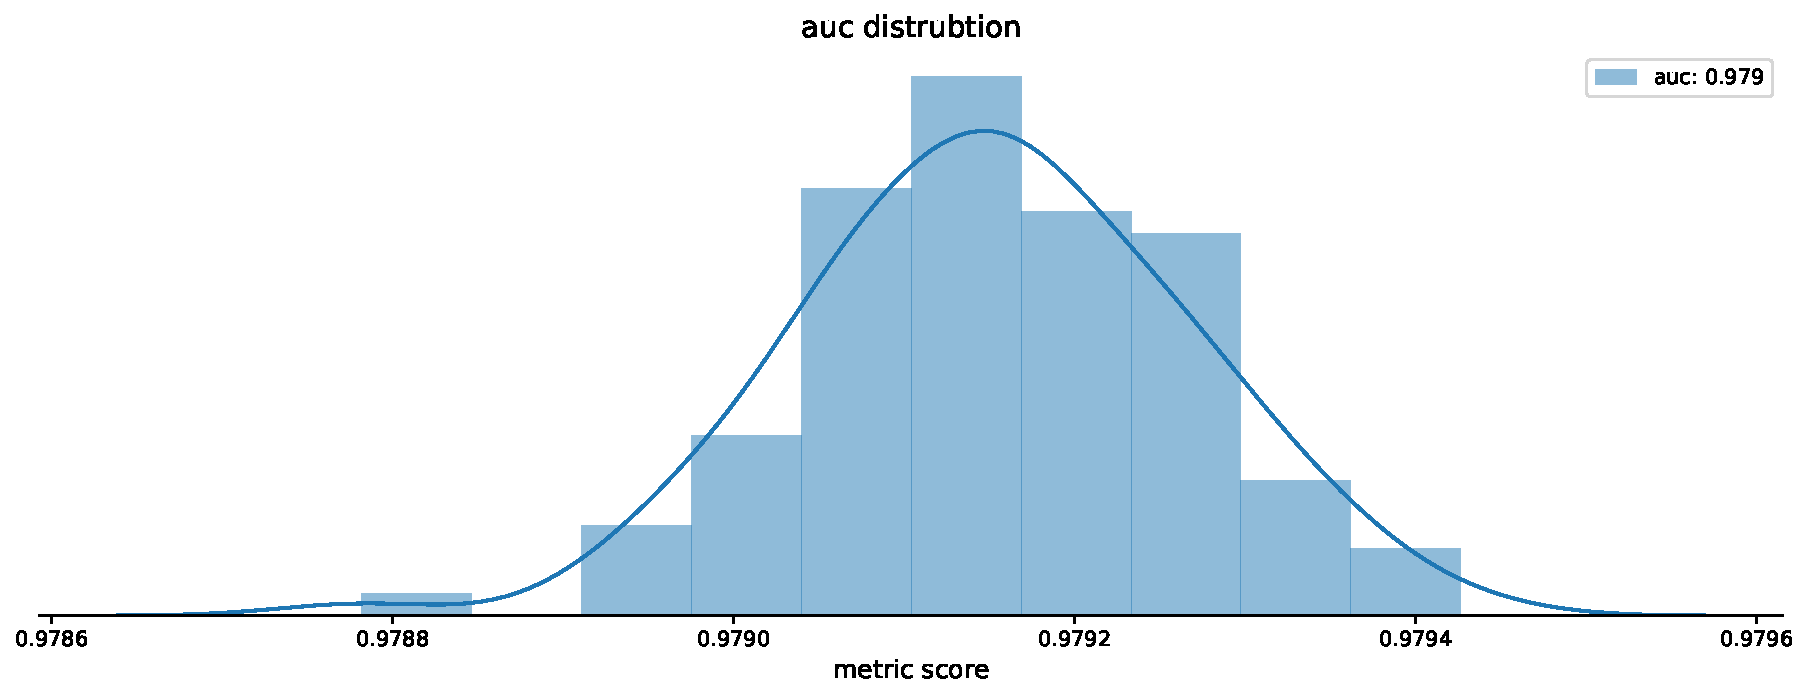
\includegraphics[scale=0.4]{auc_out_20.pdf}
    \caption{\footnotesize{auc from 100 models}}%\label{}
\end{figure}



\begin{figure}[!htb]
	\centering
	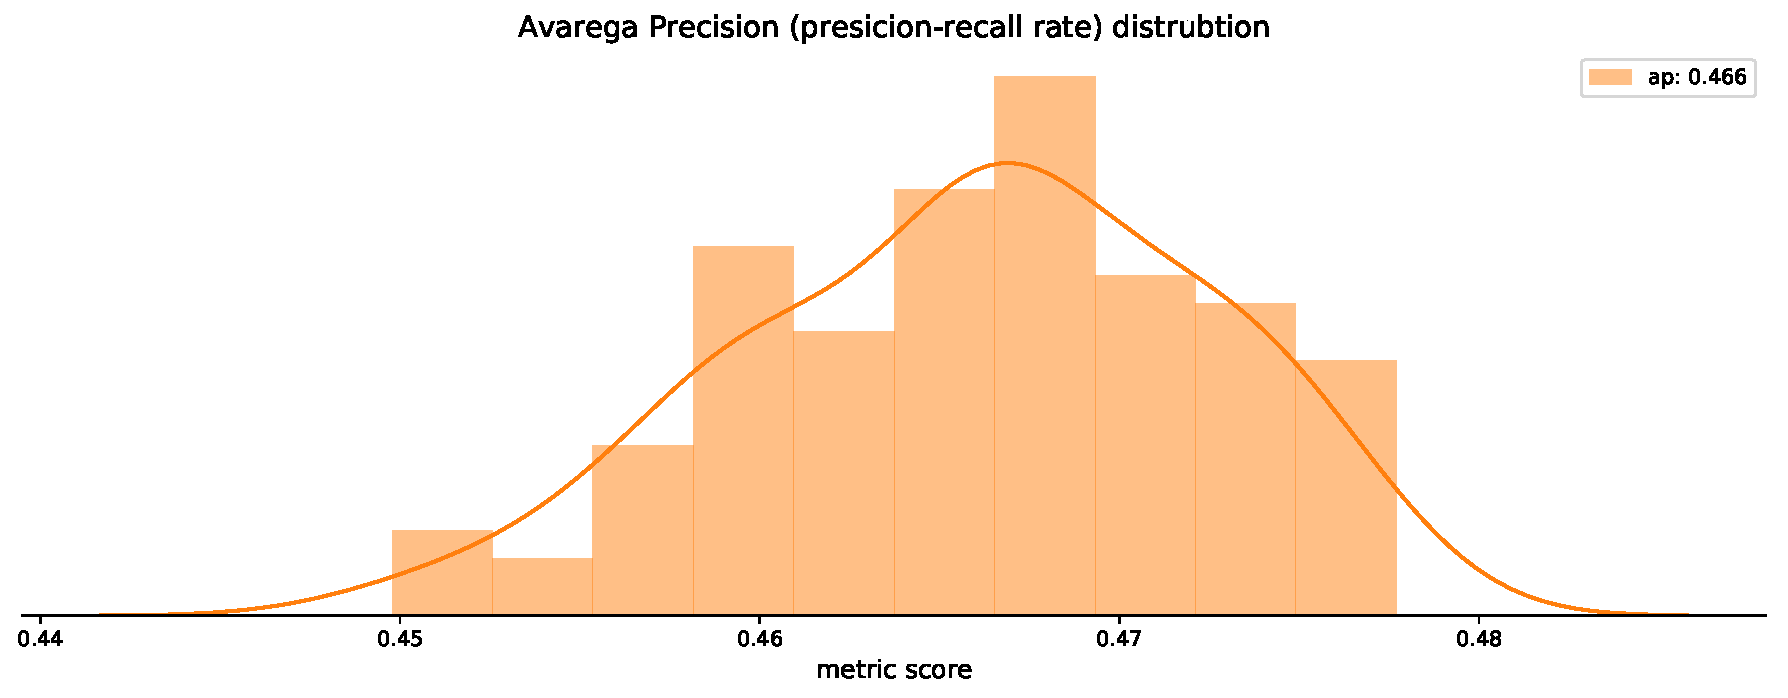
\includegraphics[scale=0.4]{ap_out_20.pdf}
    \caption{\footnotesize{Avarege Precision (presicion-recall rate) from 100 models}}%\label{}
\end{figure}


\begin{figure}[!htb]
	\centering
	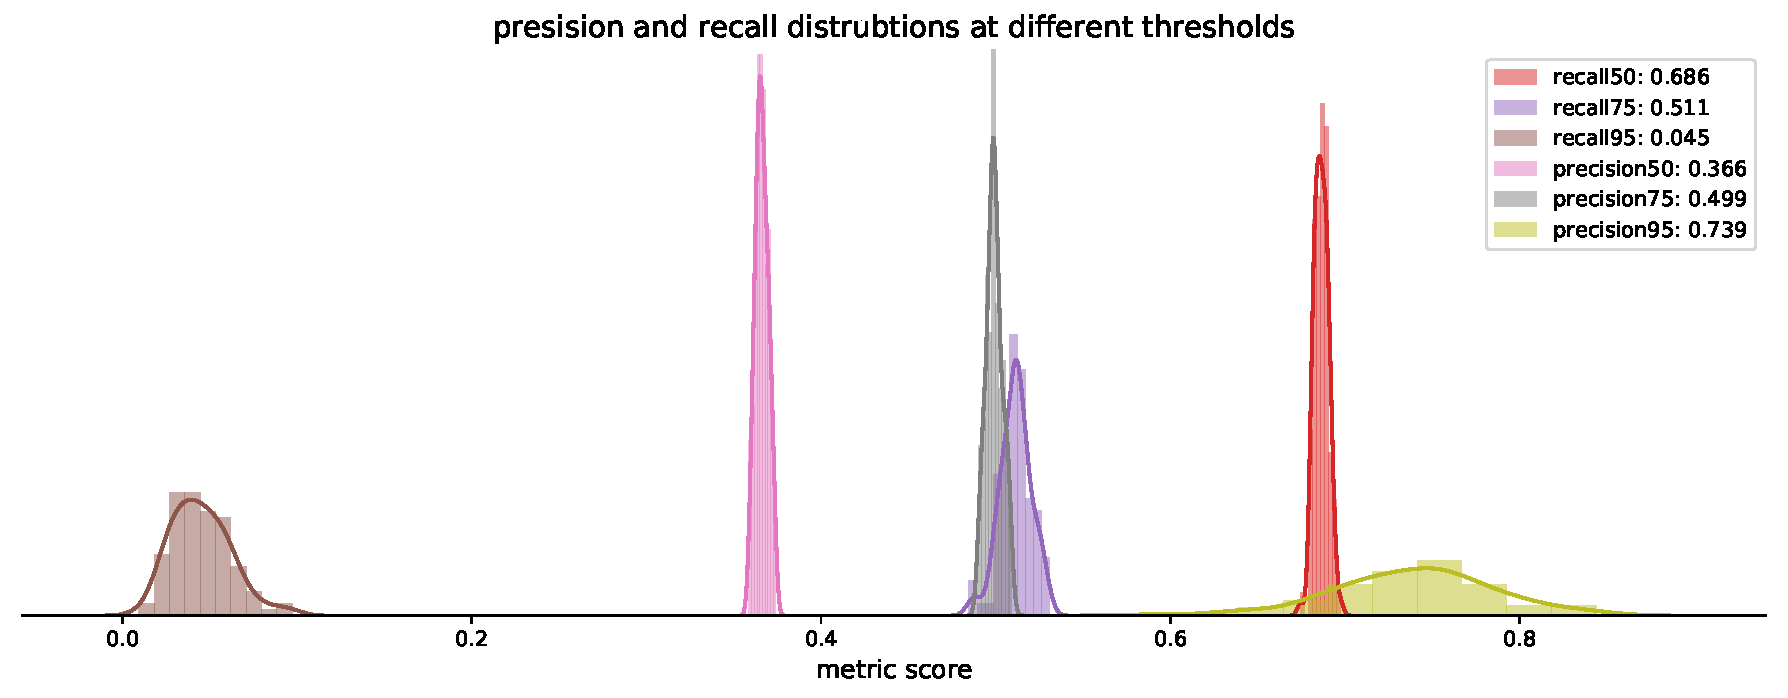
\includegraphics[scale=0.4]{recall_prec_out_20.pdf}
    \caption{\footnotesize{Precision and recall at various thresholds from 100 models}}%\label{}
\end{figure}


\begin{figure}[!htb]
	\centering
	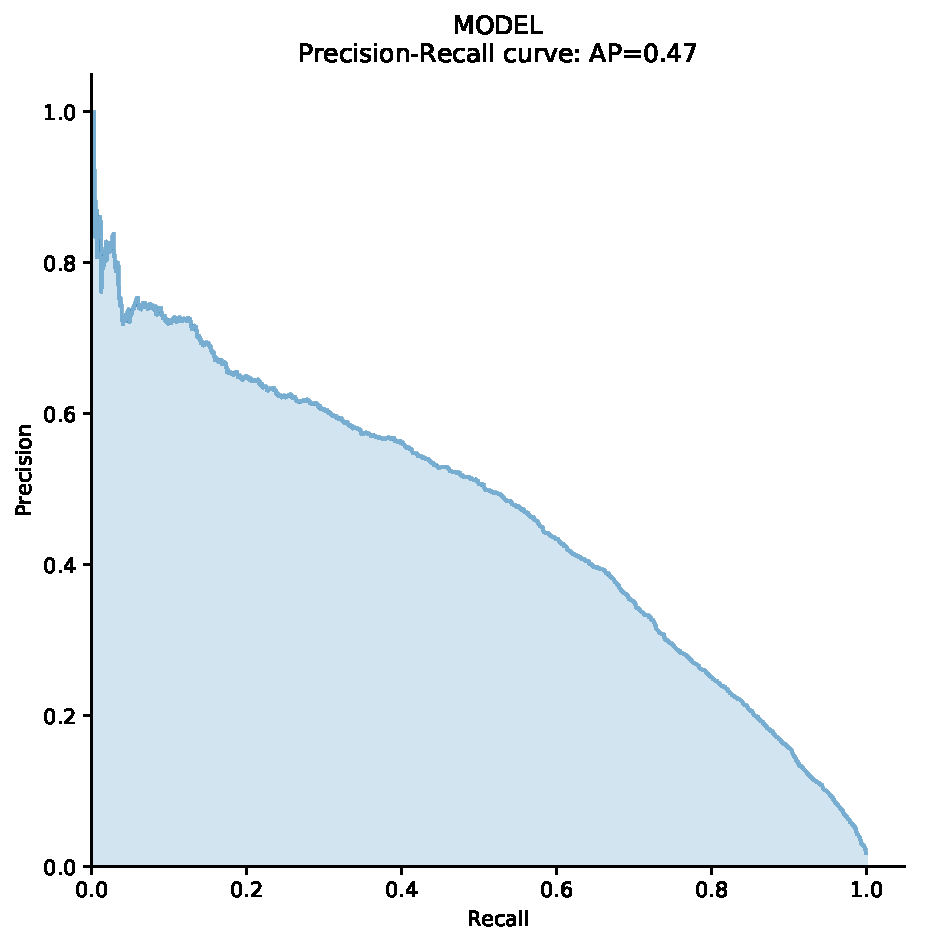
\includegraphics[scale=0.4]{prc_out_20.pdf}
    \caption{\footnotesize{Precision/Recall curve from a random model}}%\label{}
\end{figure}


\begin{figure}[!htb]
	\centering
	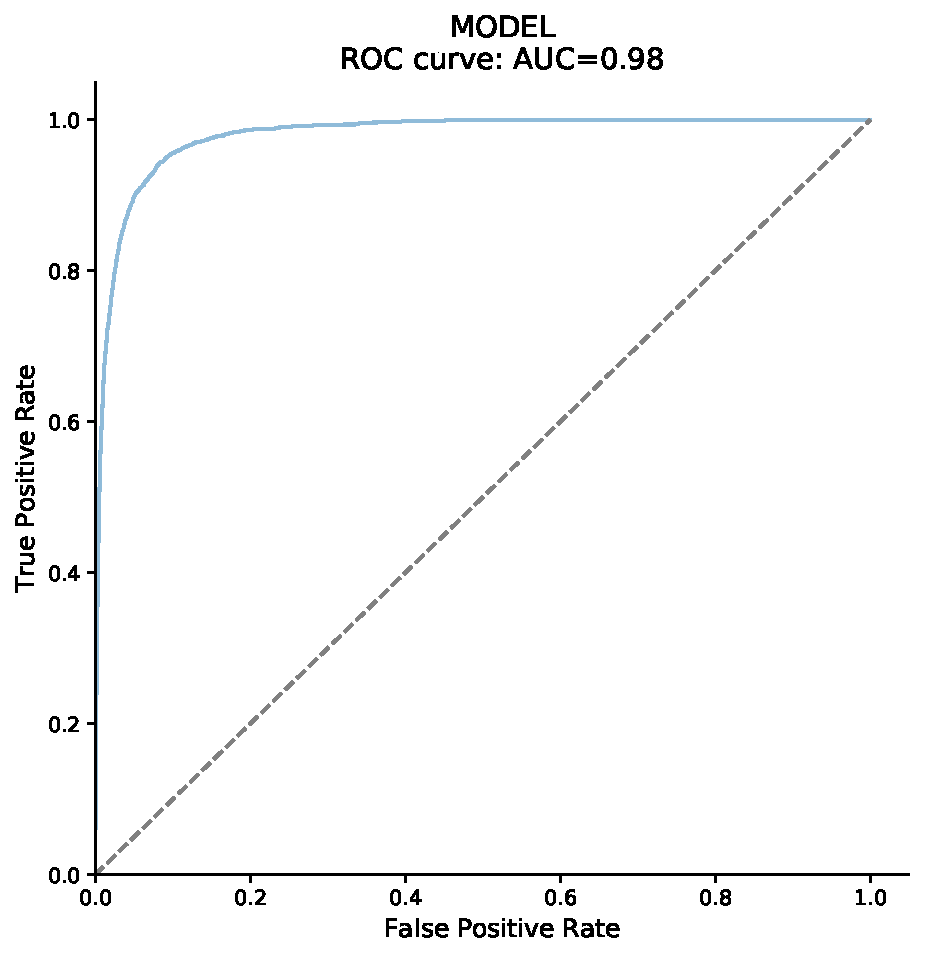
\includegraphics[scale=0.4]{roc_out_20.pdf}
    \caption{\footnotesize{ROC curve from a random model}}%\label{}
\end{figure}

\begin{figure}[!htb]
	\centering
	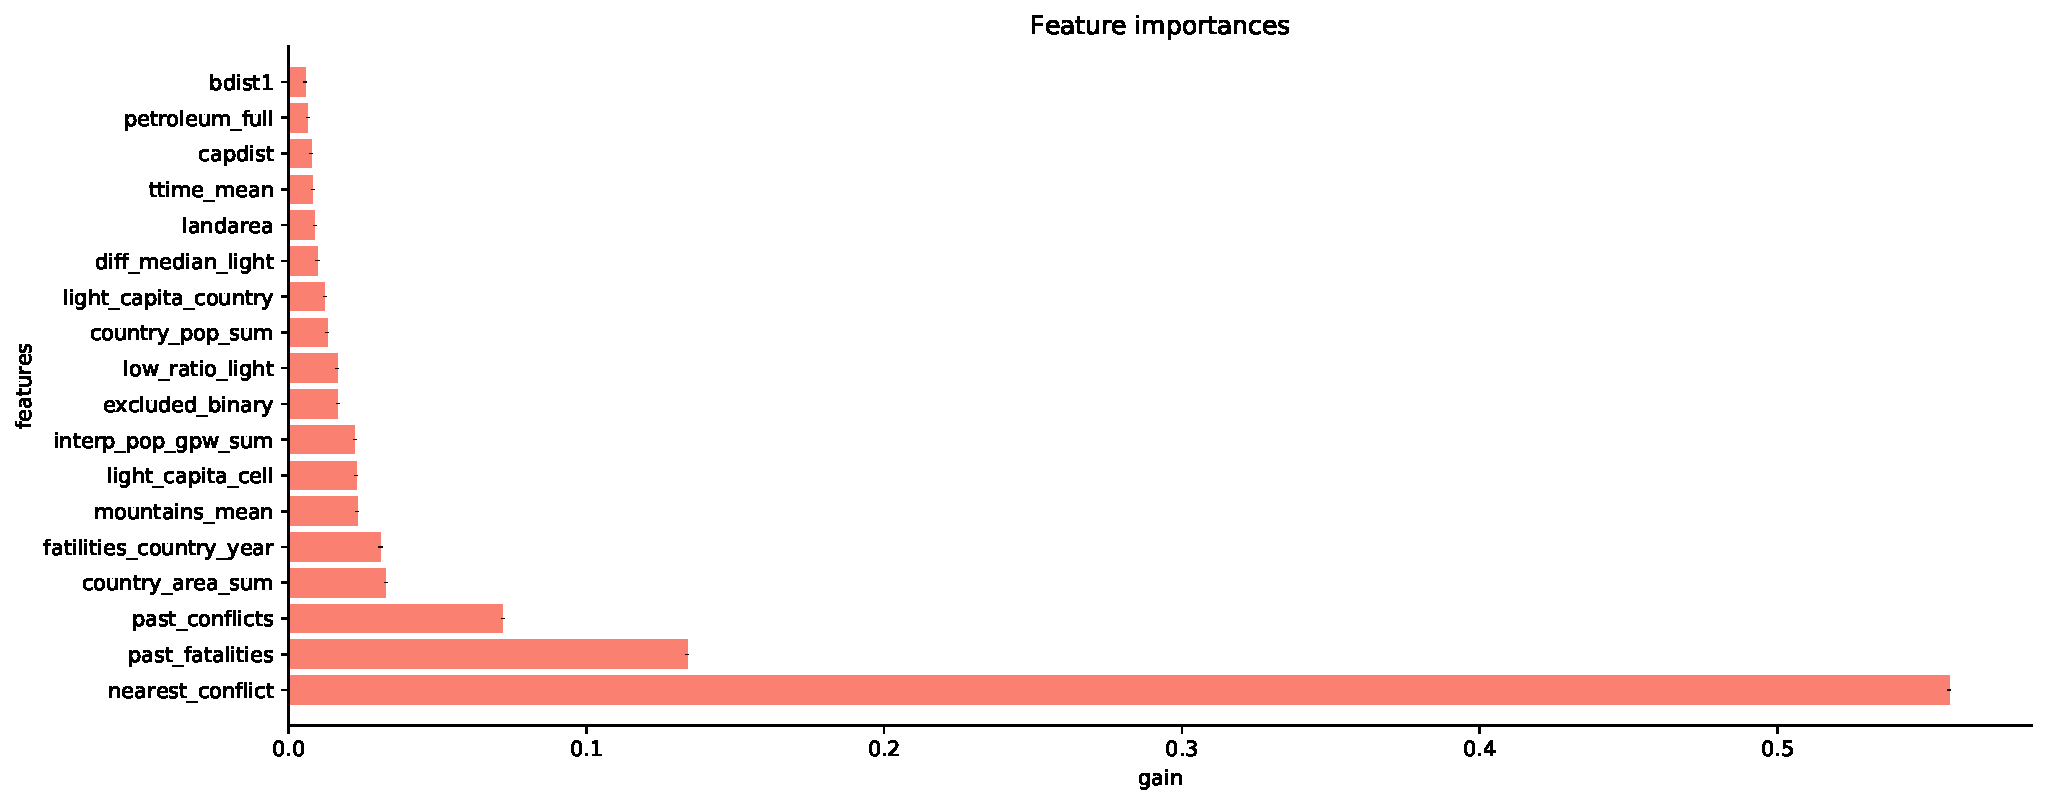
\includegraphics[scale=0.4]{feature_imp_out_20.pdf}
    \caption{\footnotesize{Feature importance across the 100 models}}%\label{}
\end{figure}

\begin{figure}[!htb]
	\centering
	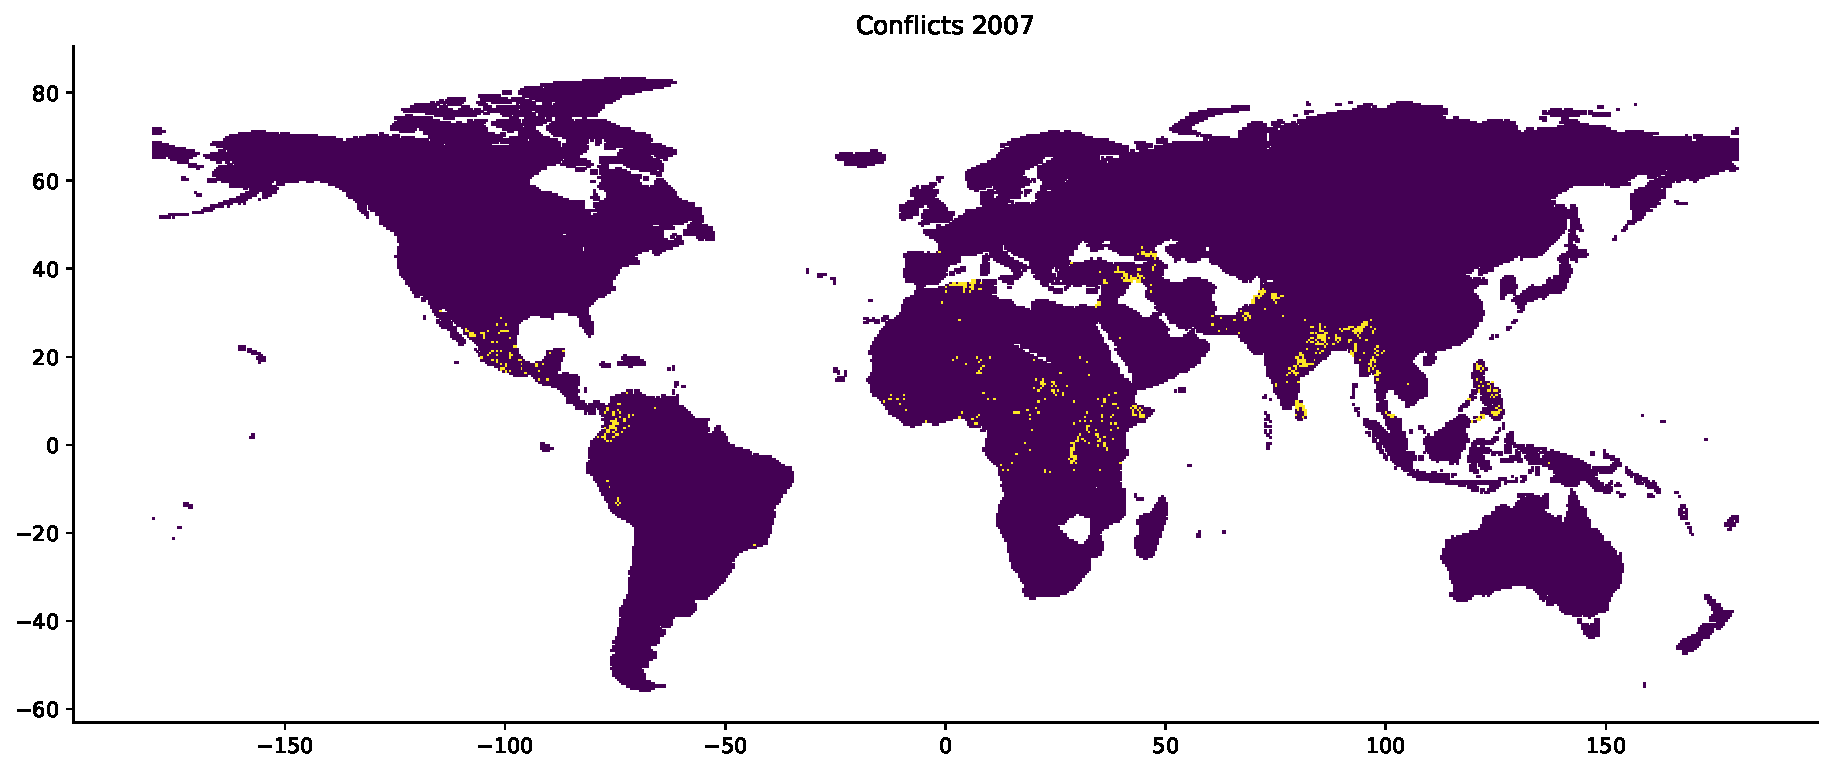
\includegraphics[scale=0.4]{conflicts_2007.pdf}
    \caption{\footnotesize{Conflicts (binary) 2007}}%\label{}
\end{figure}

\begin{figure}[!htb]
	\centering
	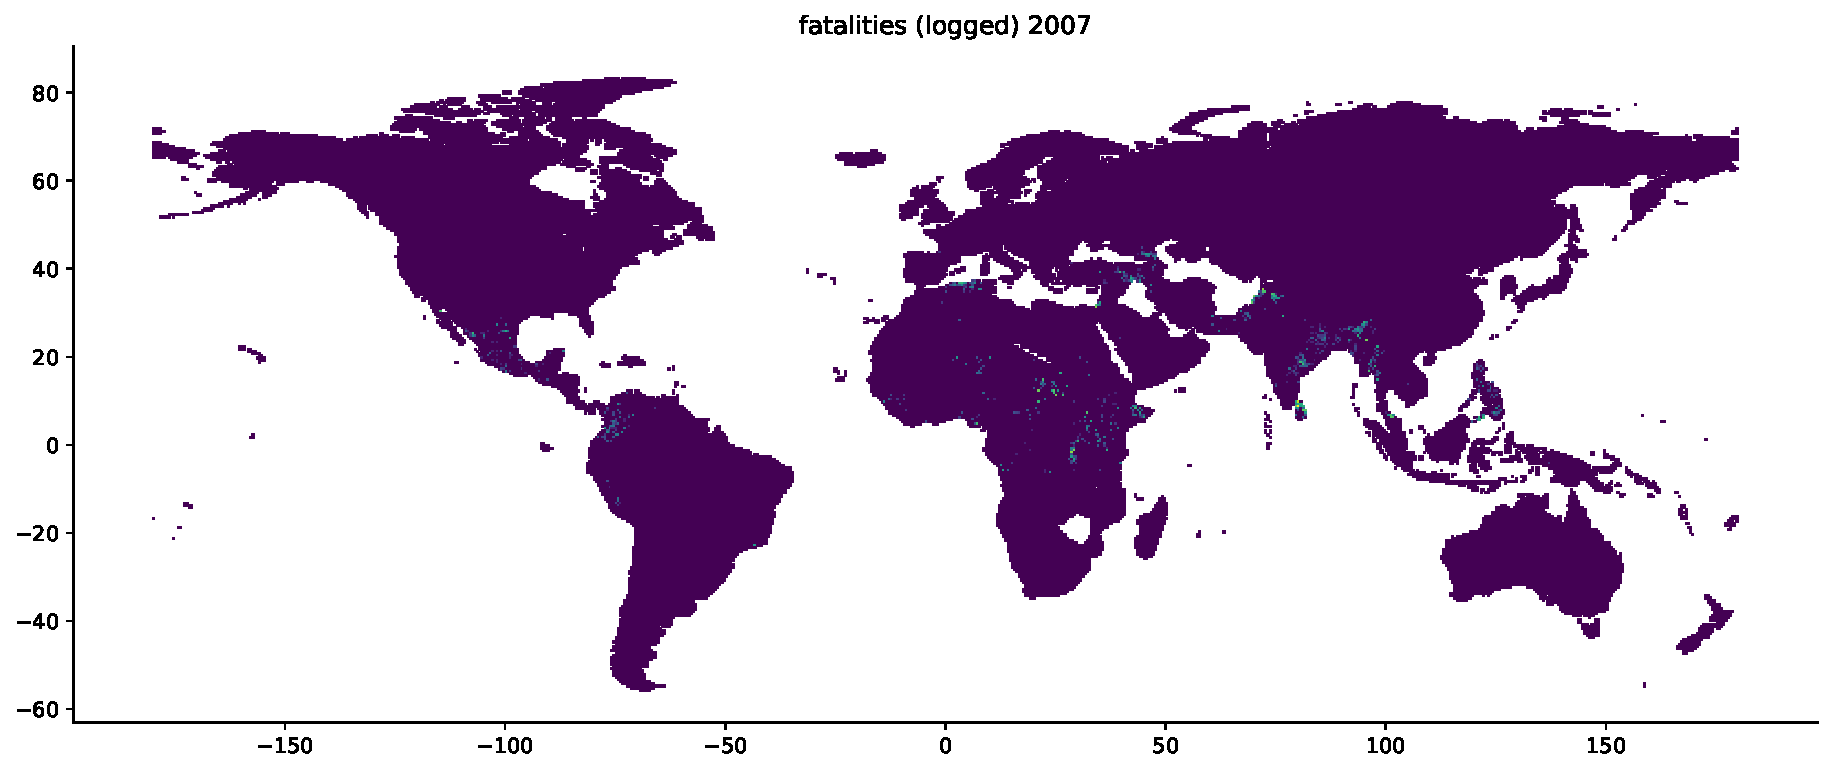
\includegraphics[scale=0.4]{log_conflicts_2007.pdf}
    \caption{\footnotesize{Fatalities (logged) 2007}}%\label{}
\end{figure}

\begin{figure}[!htb]
	\centering
	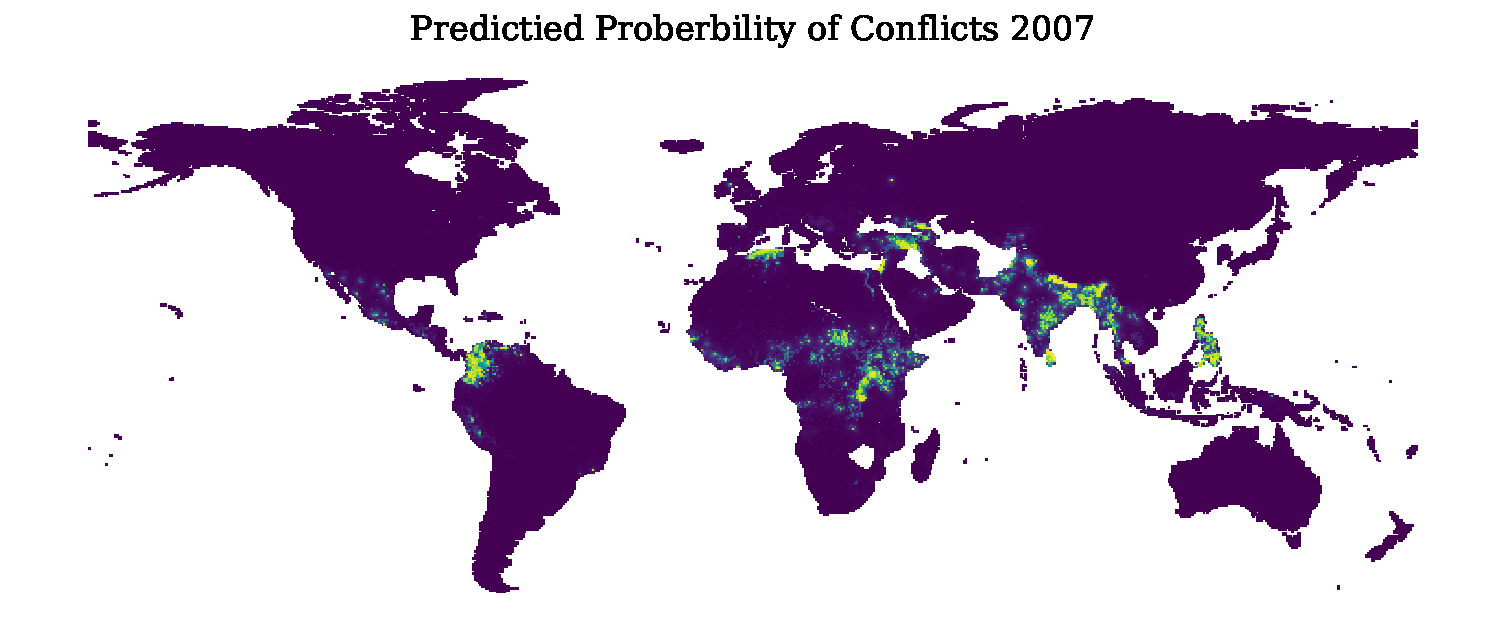
\includegraphics[scale=0.4]{pred_prob_conflicts_2007.pdf}
    \caption{\footnotesize{predicted probability of conflict 2007 - as seen we still need the bayesian correction or set the htreshold higer then 50..}}%\label{}
\end{figure}


\pagebreak

\section{Future Challenges and Improvements}
\todo[inline]{TO COME}


\section{Conclusion}
\todo[inline]{TO COME}

% \section{Feature Selection}\label{feature_selection} % ----------------------------------------

% \todo[inline]{ref til sequential feature selection; forward.}


% \section{Bayesian Multi-level Model} % ----------------------------------------

% \cite{Mcelreath_2018}, \cite{Gelman_2013}, \cite{Gelman_2006} 


% (Also introducing further methods and the model specification)

%Det faktum at der er tale om rare events gør heirarkiet uper relevatn. Du kan henvise til King and Zeng's baysiske correction men sige at du går full bayse i stedet. Bruger al information.


%Modellen skal være todelt: først logistic og så poisson elller negative-binomial. Altså hoved tingen er dit hot spot kort; hvor er der størst sandsyndlighed for at se en eller flere conflict-fatalities? Her efter tager du de observationer (hvilket cut of?) og spørger; hvor mange fatalities for venter vi her at se. Det bliver netop interessant om der er en klar sammenhæng mellem "om" og "hvor mange". Det burde der være, men lad det være et empirisk spørgsmål.

%Så du kikker ikke på individuelle variabler, men du kunne jo lave to kurve af variabler; ulighed vs. svag stat (ish) er se hvor meget hvar giver til modellen..

%HUSK: FE er også problematisk når y er binær fordi alle opservationer hvor y er invariant smides væk (jf. Cederman, Buhaug, rød 2009)

%Der er altså noget med onset og duranations (og ending). reelt skal du jo havde en model for celler hvor der ikke er konflikt; hvad er sandsyndligheden for at der opstår konflikt her? Og en model for celler med konflikt; hvad er sandsynligeden for at conflikten fortsætter?

%Måske det kan løses med en variable for "conflict last year (timeperiode = on going konflict)"? Eller endnu bedre inkooprorere det i heirarkiet?

%time since not-conflict?

%Vedr. geografi (Buhuag Gates Lujala 2009) så er du fandeme fræk hvis du kan komme med en reference til art of war

%Senere (ikke det her projekt) skal du sætte dig in i guirrilia og millitær taktikker... ellers kommer du ikke videre

%Måske en zero inflated negative binomial model alligevel er bedre end en logit?...

%Er der en interaktion mellem disttocap og disttoborder?

%Celler < lande < ongoing/not ongoing som heirarki..
%g eller bare ne variable for "time since peace". Men den variable kan jo både sættes som country og celle specific.

%eller måske: Celler < lande < ongoing/not ongoing < ever had a conflict/never had a conflict...

%for at finde ud af dit cut of for ongoing, kunne du jo lave out of smaple test.. Men du overfitter måske til data her no matter what...

% \section{From Predictions to Causality}

% \cite{King_Zeng_2001}, \cite[545]{Hegre_Sambanis_2006} ,\cite{Goldstone_2010}, \cite{Ward_Greenhill__Bakke_2010}, \cite{Schrodt_2014}, \cite[108-118,241-244,357]{Gelman_2013}, \cite[65-69]{Mcelreath_2018}.

\pagebreak

\section{Bibliography}
\bibliographystyle{apalike} 
\bibliography{conflict.bib}

\pagebreak
\section{Appendices}

All scripts can be found on : \hyperlink{https://github.com/Polichinel/Conflict_Prediction}{https://github.com/Polichinel/Conflict\_Prediction}

\subsection{Handling of random missing values}\label{missing}

\subsection{Linear interpolation from 5-years intervals}\label{interpolation}

\subsection{The Included Features - Expanded}\label{feature_expanded}


\subsubsection{Wealth and State Capacities}

 Easily one of the most robust findings in country level studies of civil wars is GDP per capita\footnote{Often logged and adjusted for purchasing power parity (ppp)} has a negative effect on the probability of civil war onset \citep{Collier_Hoeffler_1998, Fearon_Laitin_2003, Collier_Hoeffler_2004, Hegre_Sambanis_2006, Blattman_Miguel_2010} and also to some extent the conflict duration\citep{Fearon_2004, Hegre_Oestby_Raleigh_2009}.\par
 
 A number of mechanisms have been proposed linking GDP to conflict, Two have been especial prolific. The first is championed by \cite{Collier_Hoeffler_1998, Collier_Hoeffler_2004} sees GDP per capita as a proxy for opportunity-cost. that is what i given citizen have to loss by engaging in conflict. The second story draws on some insight from \cite{Skocpol_1979} and also echoes the gospel of modernization theory \citep{Lipset_1959}. Regarding the context at hand it has most prominently been presented by \cite{Fearon_Laitin_2003}. Here GDP per capita is seen as as proxy for state capacities. Simple put; weak or fragile states have low GDP per capita and these states are more conflict prone\citep[88]{Fearon_Laitin_2003}.\par
 
 A measure for GCP (Gross cell product) per capita (ppp) is included in the PRIO GRID fomr the Gecon dataset \citep{Nordhaus_2006} and this measure could be aggregated creating a feature for GDP per capita (ppp) \citep{prio_code_2015}. However the data available from the directly from the PRIO GRID only extent to 2010. Fortunately \cite{Elvidge_2009}, \cite{Chen_Nordhuas_2011} have shown that Night light emission can serve as an proxy for economic activies - especially for countries of areas with low-quality statistical systems and few or no recent population or economic censuses. \citep{Chen_Nordhuas_2011} - an approach explicitly proposed by \cite[p. 101]{Cederman_Gleditsch_Buhaug_2013} in regards to conflict studies. A ad hoc illustration of the high correlation between the two features can also be found in the appendix, \autoref{GCP_corr}\footnote{Futhermore initial test showed very limited difference between the derived features and interactions, thou the features constructed on the basis of Night Light Emission was picked more often by the sequential feature selection process in \autoref{feature_selection}.}.\par
 
 The measure of Nigth Light Emmision in the PRIO GRID is borrowed from \cite{Elvidge_2014}it extent all the way up to 2015 and calibrated as to better accommodate time series \cite{prio_code_2015}.\par % futhermore there is a interprebility problem with unpopulated cells having zero gpd per capita
 
 Thus I proceed from here with two features:
 
 \begin{itemize}
     \item Cell-year specific Night Light Emission (mean)
     \item Country-year specific Night Light Emission (aggregated mean) 
     %\item Country-year specific Night Light Emission (aggregated country median) % why? Den har du jo mest fordi du bruger den til at construere en anden var..
 \end{itemize}

% Theritical justification for the cell level? Det er en lidt bræt slutning...
Naturrally one could argue that wealth is a relative concept, which leads us to the next section.

\subsubsection{Inequality and depravation} % ------------------------------------------------------------------------

If we - for the time being - leave the Strong State proposition behind and focus on the satisfaction of the individual citizens it is only natural to argues this satisfaction should be considered a function of \emph{what we have} and \emph{what we believe we rightfully should have}. This, indeed, is the crux of Robert Gurr's \citeyearpar{Gurr_1970} Relative Deprivation Theory. Perhaps one of the most seminal\footnote{At least after Marx} takes on inequality and conflict, \cite{Gurr_1970} defines relative deprivation: 

\begin{displayquote}
\emph{"[...] as actor's perception of discrepancy between their value expectation and their value capabilities. Values expectation are the goods and conditions of life to which people believe they are rightfully entitled. Value capabilities are the goods and conditions they think they are capable of getting and keeping."} \citep[24]{Gurr_1970}. 
\end{displayquote}

While intuitively appalling, Gurr's theory was award little credit doing the haydays of comparative corss country conflict studies. Supporting statistical results failed to materialize, and the axplanation eccoed the of \cite[11]{Skocpol_1979}; injustice and misery is simply to widespread to account for the rarity of major conflicts (\citealp[p. 22]{Collier_Hoeffler_1998},  \citealp[p. 22]{Collier_Hoeffler_2004} \citealp[p. 44]{Fearon_Laitin_2003}(FLERE?)). (så lige styr på de 22 side tal der?)

% That being said, these studies have looked at larger conflicts often setting a minimum of 1000 battle related deaths per year compared to the studies at hand wich operates with a treshold of only 25 deaths per year

However, \cite{Cederman_Gleditsch_2009,Cederman_Gleditsch_Buhaug_2013} have noted that the aggregated country level features conventional used as indicators for inequality might lead to mis-specifications; that is, they do not properly measure the theoretical concept of relative deprivation or the correct mechanisms through which inequality affects conflict-propensity \citep[XX]{Cederman_Gleditsch_Buhaug_2013}. Acknowledging this critique I utilized the operationalization put forth in \cite[p. 104-105]{Cederman_Gleditsch_Buhaug_2013}\footnote{These scholars alos argues the higher conflict propensity might be fund in the other end of the inequality spectrum. That is; one could imagine a mechanism akin to relative deprivation in one end, while simultaneous at the other end, one might see well-off people wanting to secede from or take over a country if they fear to much redistribution. However, they find little statistical backing for this proposition, neither did my initial tests. Thus I only use the measures corresponding to actual Relative Deprivation}:\par

$$y_g = \textrm{country year mean}\quad ,\quad  y_c = \textrm{cell year value}$$
$$\textrm{low\_ratio} = y_c/y_g  \quad \textrm{if} \quad y_c < y_g, \quad 1 \quad \textrm{otherwise}$$

%$$\textrm{high\_ratio} = y_g/y_c  \quad \textrm{if} \quad y_g > y_c, \quad 1 \quad \textrm{otherwise}$$
Thus cells which are relatively well of compared to the mean of country takes the value 1. Cells worse of the the country mean takes a value above 1, with the magnitude of this value indicating \emph{how} severe the deprivatione is. \cite{Cederman_Gleditsch_Buhaug_2013} Uses GCP per capita (ppp) but as mentioned also suggests using night light emission, Thus I here produce ratio feature solely on Night Light emission (cell-year mean).\par

While I do appreciate this operationalization I also construct my own relative deprivation feature, which differs in a number of small but relevant ways. First we know that wealth distributions in general are highly skewed, and this is no different when we use Nigt Light Emission as indicator (se Appendix XXXX). Thus, given Gurr's original conceptualization I find it more realistic that individuals should compare themselves to the median - not the mean. That is citizens in one cell compare their living standard to the most common living standard in the country over all. In the same vein, instead of a fraction, I simply calculate the difference between the cell-year values and the country-year median. Lastly I let the value start at 0. This I do to insure that interactions create later only "activates" if the cell is actually depraved. In the case of \cite{Cederman_Gleditsch_Buhaug_2013} when a cell is not depraved, the value of a interaction takes the naked value of the other interacted feature, which is arguably somewhat imprudent. Mathematical the features is formulated as such:\par

$$y_g = \textrm{country year median}\quad ,\quad  y_c = \textrm{cell year value}$$

$$\textrm{low\_diff\_median} = y_g - y_c  \quad \textrm{if} \quad y_c < y_g, \quad 0 \quad \textrm{otherwise}$$

Thus the feature takes the value 0 if the cell is on level or above with the rest of the country. If the cell is deprived the value correspond to the difference between the country-year median and the cell value. Naturally - and as we I shall return to later - this measure and the measure by \cite{Cederman_Weidmann_Gleditsch_2011} are highly correlated, nut that does not change the fact that this last feature appears somewhat closer to the notion of relative deprivation, and more impotently it handles interactions somewhat more appropriate or at least conventional. As before the feature uses on Night Light emission (cell-year mean) as indicator for wealth.\par

\subsubsection{Ethnicity and Exclusion}


%BLIMES 2006 er også interesant her: A carefully constructed, theoretically driven empirical test has not been carried out (regaring ethnisity and civil war onset) p. 539

% Ethnicity:
%\paragraph{excluded ethnic groups} (excluded and excluded\_binary) 

Denotes the number of excluded ethnic groups (e.i. discriminated or powerless) in a given cell at a given year. The measures are originally from the GeoEPR/EPR data by \cite{Vogt_2015}. To better suit the theoretical argumentation laid forth in \cite{Cederman_Gleditsch_Buhaug_2013}(side) \citep{prio_code_2015}. I also create a dummy (excluded\_binary) which simply denote \emph{if} there are any excluded ethnic groups. 

As with inequality the link between ethnic diverse societies and conflict propensity have been ridden with disagreement and controversies. In the quantitative literature results have remained somewhat inconsistent \citep[23-24]{Blattman_Miguel_2010}. A number of studies have fund different - and sometime quite convoluted - relationships between ethnicity or discrimination and conflict \citep{Collier_Hoeffler_1998, Fearon_2004, Blimes_2006, Hegre_Sambanis_2006, Goldstone_2010}, while other studies have fund little or no trace of the connection \citep{Fearon_Laitin_2003, Collier_Hoeffler_2004}(more? CH 2004 right?).\par 

As with the problem with inequality the lack of discernible results have often been attributed to poor feature specifications, a framework not capturing the proposed theoretical mechanism and not least country aggregated data \citep{Blimes_2006, Blattman_Miguel_2010, Cederman_Gleditsch_Buhaug_2013}. Mirroring they effort concerning inequality \cite{Cederman_Gleditsch_Buhaug_2013} have recently made use of new desegregated data \citep{Girardin_2015} to closer model the theoretical mechanism proposed. Without going to much in-depth here the feature \cite{Cederman_Gleditsch_Buhaug_2013} utilizes aims to capture the effect of \emph{horizontal inequalities} as defined by \citep[31-35]{Cederman_Gleditsch_Buhaug_2013}. That is the systematic discrimination or political exclusion of and coherent ethnic group. Thou not framed in the theoretical context of horizontal inequalities \cite{Goldstone_2010} finds results supporting the argument using the Minority at Risk data from \cite{Gurr_1995}.\par

Conveniently, a measure from \cite{Girardin_2015} of how many excluded ethnic groups reside in each PRIO GRID cell is readily aviable in the PRIO GRID. To mimic the theoretical proposition lead foth in \cite{Cederman_Gleditsch_Buhaug_2013} I binarize this variable to simply indicate whether or not a given cell is inhabited by a politicly excluded or discriminate ethnic group\footnote{Also initial test did not show much prospect of incorporating the full count}. 

%\cite{Blimes_2006} etnisk factionalisering gør det meget sikre at andre facotre giver borger krig...
% Komme nede ved hierarkiet

Not surprisingly \cite{Cederman_Gleditsch_Buhaug_2013} futher finds that the properbilty of conflict gets even larger if political exclusion is followed by group deprivation, wich leads to the next feature:

\subsubsection{Deprivation and Exclusion - an Interaction}

This interaction does not need much justification; the general idea is simply that groups of humans (here specificly ethnic groups) which are both cut of from political influence and find themselves to be generally worse of then other - more influential - groups, tends to accumulate a lot of grievances. Given that few to no political solutions are available for these groups, they are reletively likely to experience conflict\cite[103-111]{Cederman_Gleditsch_Buhaug_2013}.\par

Given that I have utilized to measures of relative deprivation I also construct two interaction to be evaluated by the systematic feature selection to come:

$$ \textrm{excluded\_b\_low\_ratio\_nlights} = \textrm{excluded\_binary }\times \textrm{low\_ratio\_nlights} $$

$$ \textrm{excluded\_b\_low\_median\_diff\_nlights} = \textrm{excluded\_binary }\times \textrm{low\_median\_diff\_nlights} $$

One very relevant difference here is that the feature from \cite{Cederman_Gleditsch_Buhaug_2013} takes the plain value of 'excluded' $\in {0,1}$ if the cell is not deprived while the interaction only takes the value of 0 if 'excluded' takes the value zero. As mentioned I find this somewhat messy and statistically it makes it harder to determined the effect of 'excluded' in it self and the interaction. Naturally this is an issue I return to in \autoref{feature_selection}.\par

\subsubsection{Population size and density} 

Returning to a variable with a rather flawless record regarding conflict onset we have "country population size" \citep{Collier_Hoeffler_1998, Fearon_Laitin_2003, Collier_Hoeffler_2004, Hegre_Sambanis_2006}\footnote{though see \cite{Goldstone_2010}}. Furthermore \cite[287]{Fearon_2004} also finds that country population is correlated with longer civil wars.\par

Lastly when it comes to disaggregated grid data, the "grid population size" also seems a rather robust predictor \citep{Buhaug_2010, Cederman_Gleditsch_Buhaug_2013}\footnote{Though see \cite{Hegre_Oestby_Raleigh_2009}}. Thus, whether the features influence conflict duration is more disputed \citep{Collier_Hoeffler_1998, Fearon_2004}. The most common implementation is to use a log transformed version of the country or grid population count\footnote{Though \cite{Collier_Hoeffler_1998} use the plain count in 10.000's} which is also implemented in the project at hand.\par

%(Det er vel endnu mere relevant for gridded? større variation?)(det er også log den FS finder, så måske du skal smide den anden væk..)

One very simple explanation might be the various definitions of conflict and civil war used throughout the litterature. These definitions almost always refer to some minimum fatalities count [eks and refs]. Naturally high population counts makes these threshold relativly less restrictive.\par

There are however also more theoretical propositions for the relationship. One being that conflict mediation becomes inherently more difficult as social systems and societies grow \cite[p- 271-272]{Diamond_1998}.\par

Initial I include features for cell-year population, aggregated country-year population and corresponding population densities:

$$\textrm{grid\_pop\_dens} = \frac{\textrm{grid\_pop}}{\textrm{grid\_area}}$$

$$\textrm{country\_pop\_dens} = \frac{\textrm{country\_pop}}{\textrm{country\_area}}$$

Which leads to the last included interaction concerning excluded ethinic groups.\par 

\subsubsection{Density of the Excluded - Interaction} %----------------------------------------------------------- 

(excluded\_pop, excluded\_b\_pop) 

One more drawn directly from \cite{Cederman_Gleditsch_Buhaug_2013} disaggregated study conserns the interaction between population size and group exclusion. the Auothors construct an interaction between the size of the cell population and their feature for excluded ethnicities \citep[73-78]{Cederman_Gleditsch_Buhaug_2013}. Assuming that the size of the excluded population is at least positively correlated with the total cell population this feature captures the density of the excluded population. 

$$ \textrm{excluded\_b\_pop}  = \textrm{excluded\_binary} \times \textrm{cell\_pop}  $$

The theoretical argument is simply that it is not larger population but larger excluded populations that drives the relationship between conflict and population size \citep[69-74]{Cederman_Gleditsch_Buhaug_2013}.

\subsubsection{Geography and Accessibility} %------------------------------------------------------------------

\paragraph{Accessibility} As noted earlier, a strong state have often been presented as the prime inhibitor of internal conflicts. Naturally though, the strength of state must be considered relative to the territory over which it claims sovereignty - both in regards to size and permeability. \cite{Fearon_Laitin_2003} pointed to rough terrain and mountains as natural obstacles hindering effective projection of state power. Following this example \cite{Hegre_Sambanis_2006} concludes that a feature for rough terrain is found to robustly positively correlated with civil war across a large number of model specifications.\cite[526-529]{Hegre_Sambanis_2006}\footnote{Though see \cite{Goldstone_2010}}. The Prio Grid includes a readily available feature measuring the proportion of mountainous terrain within the cell based on \cite{Blyth_2002} wich I utilize.\par

Another natural hindering for projecting state power is sheer distance \citep{Fearon_2004, Buhaug_Gates_Lujala_2009, Cederman_Buhaug_Roed_2009, Buhaug_2010}. The argument is straight forward:

%\cite{Buhaug_2010} : cap dist
\begin{displayquote}

\emph{"The projection of power across distance comes at a cost. [...] In particular, large hinterlands and isolated peripheries are favorable to insurgency. In sum, this suggests that large countries are relatively more exposed to intrastate conflict"}\cite[113-114]{Buhaug_2010}

\end{displayquote}

A number of interesting features could be derived from Buhuag's assertion above (and the paper in general). What I have included is the distance to the nations capital\footnote{The measure utilized by \cite{Buhaug_2010}}, the travel time to the nearest major city, and the total size of the country\cite{prio_code_2015}.

%me: and also the grid cells are not the same size..


\subsubsection{Trans-boarder Influences} %--------------------------------------------------------------------

A number of different mechanism have been proposed and explored \citep[29-30]{Blattman_Miguel_2010}, the one explored here is rather simple and follows \cite{Hegre_Sambanis_2006} [TJEK IGEN!]. blabla

Der er vel også lidt en tråd til Conflict dispersion....

de to mål og hvorfor du inkoorporere begge.

\paragraph{bdist1}  
\paragraph{bdist3}

% hvorfor samler du dem ikke bare i et mål? bare pluser dem sammen? 

This is a very rough measure and is arguably a bit far removed from any specific theoretical concept, but for this preliminary project the measures will have to do.

\subsubsection{Urban contra Rural Theater} %--------------------------------------------------------------------

Ja, hvad er din teoritiske begrundelse her? går du tilbage til litteraturen om democratiske sammenbrud? Noget med at der er mere undertrykkelse i land områder hvilket leder? (Boix, Robinson, Acemogul...) Til grievences? Eller omvendt er det lettere at mobilisere i byerne?

Det trækker også lidt på det accesability du har snakket om tidligere... Son of the soil..

\paragraph{interp\_urban\_ih} her henter du også viden fra democratic breakdown lit.  
\paragraph{interp\_agri\_ih}  her henter du også viden fra democratic breakdown lit.  og Skocpol


\subsubsection{Prime Commodities and the Recourse course} %-----------------------------------------------------------

først: prime comoditeis in general:
\cite{Collier_Hoeffler_1998, Collier_Hoeffler_2004}

find no impact of prime comm. \cite[76]{Fearon_Laitin_2003} does find inpact of oil \cite[84-86]{Fearon_Laitin_2003}


Kikker videre på prime comm. \cite{Fearon_2005}, ( or Natural reasources) \cite{Ross_2004}

Og sons of the soils \cite{Fearon_2004}, men så skulle du lave nogle interactioner med excluded..

\cite{Buhaug_2010} Oil disaggregated

As such, the soil feature here included is a binary indicator of whether oil is know to be available for extraction in a given cell at a given year. % (petroleum\_full). 

\cite{Hegre_Oestby_Raleigh_2009} : also a bit on prime Comm




\subsubsection{Inertia, dispersion, traps and time trends} %---------------------------------------------------------------

%Havd gør du? Hvordan og hvornår bliver dette inkoorporet i modellen?

Conflict, inertia, trap, conflict dispersion, time trends ect

\cite{Collier_Hoeffler_2004} : linear DECAY term since last conflict.

\cite{Goldstone_2010} : conflict ridden neighbourhood.

\cite{Hegre_Sambanis_2006} : which we model as a DECAY function of time at peace

"Among others, we include a decay function proxregc of the Polity
durable variable, which measures the number of years since an institutional change
that leads to a minimum of three points' change on the Polity index."

"In a review of the quantitative literature on civil war, Sambanis
(2002) identified the following three core variables that are almost always included
in models of civil war onset: the natural log of population (Inpop), the length of
peacetime until the outbreak of a war (pt8, which we model as a decay function of
time at peace), and the natural log of per capita gross domestic product (GDP) in
constant dollars (Ingdp)."

%Neighbourhood effect of civil wars - right? Ud over spatial autocorrolation kan du modllere det på både lande og celle niveau - det vill fylde meget mind, men også smide meget information væk...

%har også argumenter vedr. mange etniske grupper og faldende risiko for conflict... Og det har C og H 1998 jo også

%også om hvorfor prediction er viktigt (p. 545) - se også Schrodt xxxx, Goldstone 2010 og Greenhill, Bakke et al.. XXXX

%"The "neighborhood at war" (natwar) variable has robustly positive estimates for
%both conflict variables, lending support to hypotheses regarding the significance of
%diffusion and contagion effects in civil war"

\cite{Cederman_Gleditsch_Buhaug_2013} Number of previous conflicts



\subsubsection{Notable Absentees}\label{notable_absentees} %---------------------------------------------

Notable missing: infant mort, political system and intra elite conflict... \citep{Goldstone_2010} Past conflicts (contry and cell level..) (conflict trapp, Coiller ect) ... Trans boarder thing.. Downgraded... \citep{Cederman_Gleditsch_Buhaug_2013}

\cite[119-142]{Cederman_Gleditsch_Buhaug_2013}: Du har border, men måske er mekanismen ikke rigtigt specificeret. det er trans-boarder-ethnic-kin

\cite{Goldstone_2010} : Infant mortality deviant from global mean, factionalisation (political system), state led discrimination (nej, den e rjo lidt med igennem excluded), conflict ridden neighbourhood(er med på celle basis gennem nearest ish). p: 


%\section{Data Handling and exploration}
% Nej! det skal ind under data sources of features.


\subsection{GCP and Night Light Emission}\label{GCP_corr}



%\section{ref tjeck..}
%\cite{Fearon_Laitin_2003}
%\cite{Collier_Hoeffler_2004}
%\cite{Fearon_2004}
%\cite{Ross_2004}
%\cite{Fearon_2005}
%\cite{Hegre_Sambanis_2006}
%\cite{Kalyvas_2007} % Hvad med den her? Den kan ellers bruges massere steder!!!
%\cite{Vreeland_2008}  % Har du brugt den her? -> eller nævn i abseentess afsnitet
%\cite{Cederman_Gleditsch_2009}
%\cite{Cunningham_Gleditsch_Salehyan_2009}
%\cite{Hegre_Oestby_Raleigh_2009}
%\cite{Buhaug_Gates_Lujala_2009}
%\cite{Cederman_Buhaug_Roed_2009}
%\cite{Beardsley_McQuinn_2009} % Har du brugt den her?
%\cite{Weidmann_2009}
%\cite{Goldstone_2010}
%\cite{Blattman_Miguel_2010}
%\cite{Buhaug_2010}
%\cite{Cederman_Weidmann_Gleditsch_2011}
%\cite{Cederman_Gleditsch_Buhaug_2013} (only read the conclusion)

\end{document}
